%%%%%%%%%%%%%%%%%%%%%%%%%%%%%% Preamble 
\documentclass[titlepage]{scrartcl} 
\usepackage{amsmath,amssymb,amsthm,fullpage} 

\usepackage{graphicx} % support the \includegraphics command and options
\usepackage{caption}
\usepackage{subcaption}

\begin{document}
\pagenumbering{gobble}

\pagestyle{plain}
\pagenumbering{arabic}

%%%%%%%%%%%%%%%%%%%%%%%%%%%%%% Heading 
	\title{EE/CS 52 SoPC Digital Oscilloscope}
	\subtitle{User Manual}
	\author{Santiago Navonne} 
	\date{June 2014} 
	\maketitle

	
%%%%%%%%%%%%%%%%%%%%%%%%%%%%%% Body
	\section{Introduction}
	This guide describes the characteristics and operation of the EE/CS 52 System-on-Programmable-Chip (SoPC) Digital Oscilloscope.\\
	
	The device is a color digital oscilloscope that allows the user to measure and display voltages over time with a bandwidth of 9.5 MHz (sampled at 19 megasamples per second). The system supports common features such as manual, one-shot, and automatic trigger. Additionally, various sweep rates, trigger levels, trigger slopes, and positive delays can be configured from a user interface on the display. A grid or axes can be overlaid on the waveform for measuring convenience, and a cursor can be used to easily report the actual value.
	
	\section{Specifications}
	The system's characteristics are described in the following table.

	\begin{center}
    		\begin{tabular}{ p{5cm} p{10cm} }
		Display & 3.5 inch, 480x270, color Liquid Crystal Display (LCD) \\
		User Input & Two knobbed rotary encoders with push-buttons \\
		\\ \hline \\
		Sample Rates & 53, 105, 211, 500 ns; 1, 2, 5, 10, 20, 50, 100, 200, 500 $\mu$s; 1, 2, 5, 10, 20 ms \\
		Sampling Resolution & 8 bits \\
		Input Voltage Range & -10.0 V to +10.0 V \\
		Trigger Level Resolution & 7 bits \\
		Trigger Slope & Positive or negative \\
		Trigger Delay & Up to 4,294,967,295 sample times (i.e. 430 s at 100 ns sample rate) \\
		Captured data points per sample & 480
		\end{tabular}
	\end{center}
		
	\section{Layouts}
	Users only need to interact with three sections of the printed circuit board: the power connector, the probe connector, and the rotary encoders. All three sections are highlighted in Figure~\ref{fig:user_board_layout}. Additionally, users can reset the system using the highlighted Reset button. \\

	\begin{figure}[h]
	\includegraphics[width=\textwidth]{img/user_board_layout.png}
                	\caption{Position of user interface elements on printed circuit board.}
               	\label{fig:user_board_layout}
	\end{figure}

	The user interface displayed on the LCD is shown in Figure~\ref{fig:user_screen_layout}, and presents three different parts: the most recent trace with the associated grid or axes selected through the menu is displayed in the background, the trace shown in green, with the cursor in red when enabled, and the scale in gray; the cursor's text displaying the currently measured value is shown in the top-left corner; and the menu, when displayed by pressing the push-button on either rotary encoder, appears in the top right corner.

	\begin{figure}[t]
	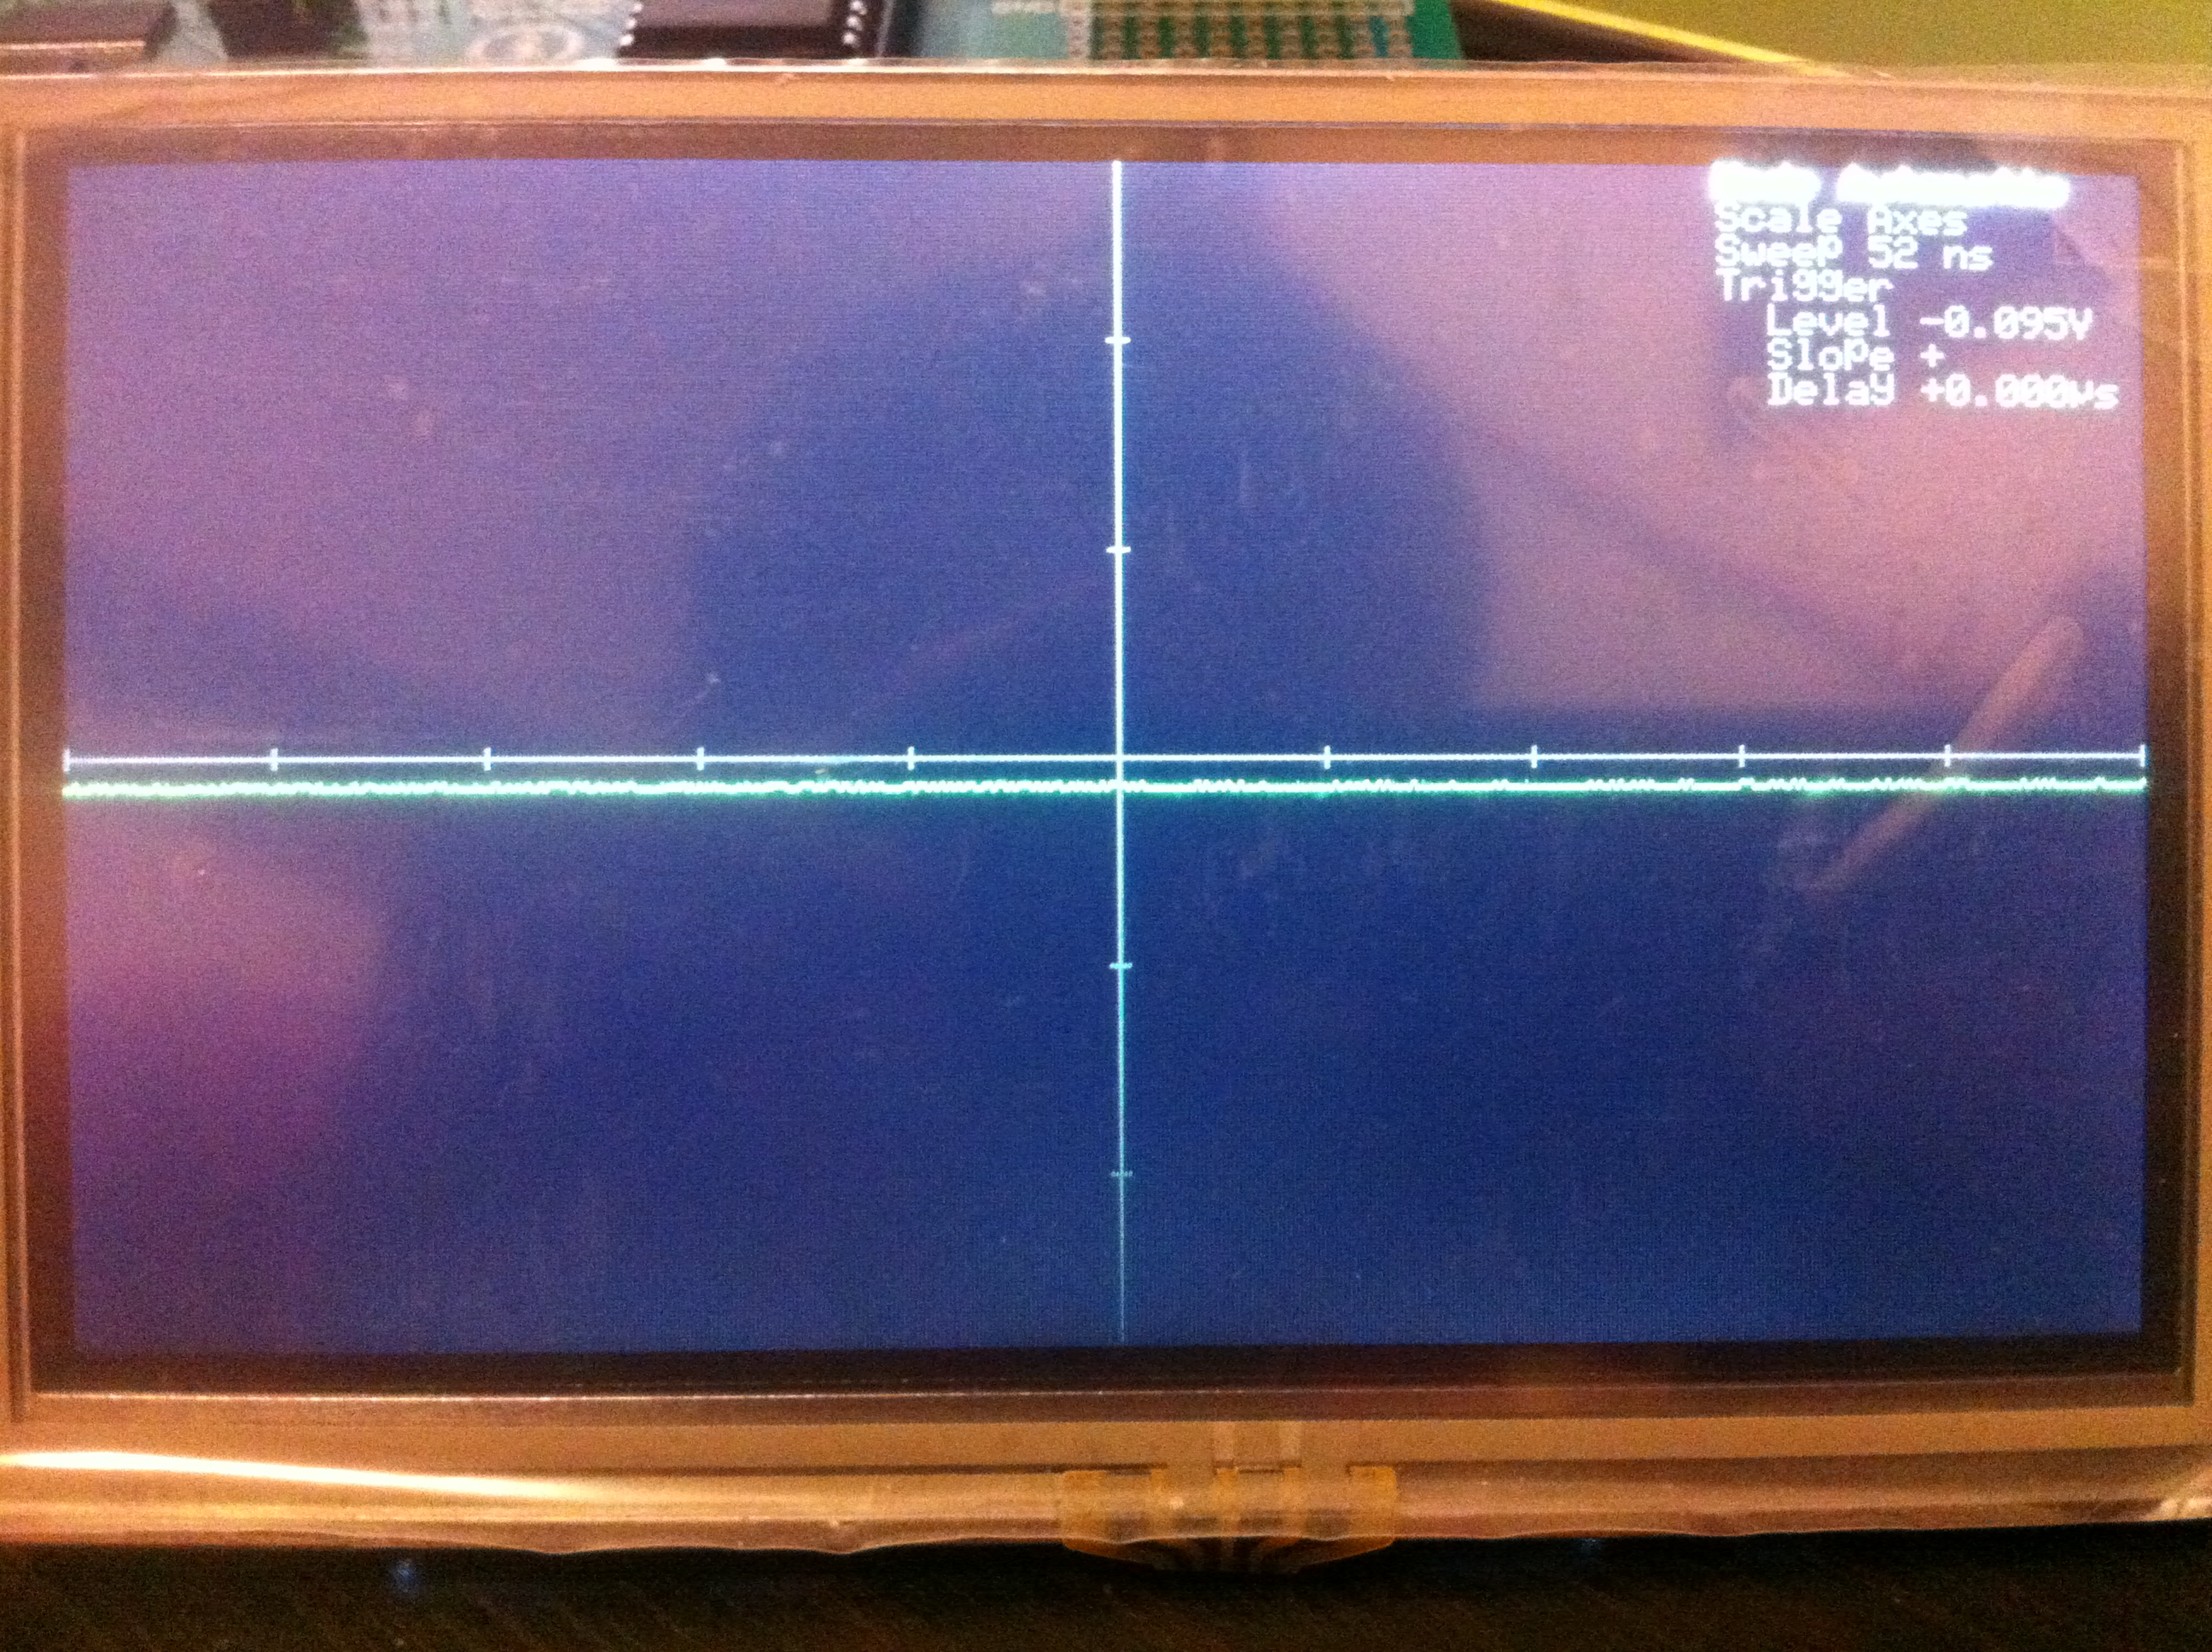
\includegraphics[width=\textwidth]{img/user_screen_layout.jpg}
                	\caption{Position of user interface elements on display.}
               	\label{fig:user_screen_layout}
	\end{figure}

	\section{Setup}
	To start the system, simply connect a compatible power supply to the DIN-5 power connector on the printed circuit circuit board. The system thus starts in one-shot trace mode with a sampling rate of 100 ns, a mid-level trigger (halfway between the minimum and maximum trigger levels) with no delay and positive slope, and with the menu displayed and scale set to axes. At this point, the device is ready for use: the signal to be measured can be connected to the BNC probe connector at any point in time (``hotplugging" is supported).
	
	\section{Usage}
	The user can change the oscilloscope configuration via the two rotary encoders in the bottom-left corner of the printed circuit board. Note that only one concurrent action is supported: only one knob should be operated at a time, and the buttons should not be pressed while any one of them is being rotated (or vice versa).\\

When the menu is being displayed, the selected option is always highlighted in white, while other options are displayed in gray. Rotating the Menu Navigation (left) knob clockwise moves down the menu, and rotating it counter-clockwise moves up; rotating the Option Selection (right) knob clockwise increments or changes the value of the configured option, while rotating it counter-clockwise decrements it. Changes take effect immediately. The menu can be hidden and shown at any time by pressing the push-button on either rotary encoder. The menu entries are described in more detail below.\\

The \textit{Mode} menu entry can be set to Mode Normal, Mode Automatic, or Mode One-Shot. In Mode Normal the scope waits for another trigger after every retrace. In this mode new traces are captured as fast as the system can redraw the waveform. Mode Automatic works the same as Mode Normal if there are trigger events; but if no trigger event occurs after 10 ms, the scope triggers automatically without a trigger event occurring. In Mode One-Shot the scope triggers only once and then holds that trace on the screen. It does not look for another trigger event until the Trigger menu item is selected and the Option Selection rotary encoder is rotated.\\

The \textit{Scale} menu entry can be set to Scale Axes, Scale Grid, or Scale Off. If the scale is set to Scale Axes, the x and y axes are displayed along with the trace. If the scale is set to Scale Grid, an x-y grid is displayed along with the trace. If the scale is set to Scale Off, no axes or grid are displayed.\\

The \textit{Sweep} menu entry sets the sweep rate (in time per sample) for the scope. Possible settings are: 52, 104, 208, and 500 nanoseconds, and 1, 2, 5, 10, 20, 50, 100, 200, and 500 microseconds, and 1, 2, 5, 10, and 20 milliseconds (per sample).\\

The \textit{Trigger} menu entry re-arms the trigger for the scope in one-shot mode. Any time it is selected and the Option Selection encoder is rotated the scope trigger is re-armed and a new trace will then be captured once the trigger conditions (level and slope) are met.\\

The \textit{Level} menu entry sets the trigger level. It can be set to any value from the most negative input voltage to the most positive in 128 steps.\\

The \textit{Slope} menu entry is either Slope + or Slope - and determines whether the scope is triggered on a positive or negative slope respectively.\\

The \textit{Delay} menu entry determines the trigger delay. It sets the time after the trigger event at which the trace will start. It may be set to any value from the minimum delay to the maximum delay times the sample rate and it is displayed as a time.\\

	\section{User Input}
	The user input section consists of two rotary encoders located in the lower-left corner of the printed circuit board, as shown in Figure~\ref{fig:user_board_layout}. The function of these knobs are summarized in the table below. Additionally, the system can be reset by pressing and releasing the Reset button.

	\begin{center}
    		\begin{tabular}{ p{3cm} p{3cm} p{10cm} }
		 Menu Navigation & Push-button & Display or hide the menu. If the menu is not being displayed, rotating either rotary encoder has no effect. \\
		 & Clockwise & Move the cursor down, if not already at the bottom menu item. If at the bottom, do not move the cursor.  \\
		 & Counter-Clockwise & Move the cursor up, if not already at the top menu item. If at the top, do not move the cursor. \\
		\\ \hline \\
		Option Selection & Push-button & Display or hide the menu. If the menu is not being displayed, rotating either rotary encoder has no effect. \\
		 & Clockwise & Change the currently selected (highlighted) menu item. Go ``forward" through the list of possible settings. If at the ``end" of the list, don't change the current selection. \\
		 & Counter-Clockwise & Change the currently selected (highlighted) menu item. Go ``backward" through the list of possible settings. If at the ``beginning" of the list, don't change the current selection. \\
		\end{tabular}
	\end{center}

	
	\end{document}